\documentclass[preprint,11pt,times,number,sort&compress]{elsarticle}
\usepackage[margin=0.89in]{geometry}
\journal{Information Sciences}
\usepackage[T1]{fontenc}
\usepackage{microtype}
\usepackage{amsmath,amssymb,mathtools,amsthm}
\newtheorem{proposition}{Proposition}
\usepackage{booktabs,tabularx,array,multirow,threeparttable}
\usepackage{graphicx,xcolor,enumitem,caption}
\usepackage{placeins,needspace,setspace}
\usepackage{lineno}
\usepackage[hidelinks]{hyperref}
\usepackage[nameinlink,noabbrev]{cleveref}
\usepackage{xurl}
\hypersetup{pdfauthor={Runze Zhu; Guanfeng Li},pdftitle={PAIR: Compiling reference- and source-qualified comparisons from incomplete molecular screens}}
\newcommand{\method}{PAIR\xspace}
\newcommand{\pairkg}{PAIR-KG\xspace}
\newcommand{\paireval}{PAIR-Eval\xspace}
\newcommand{\R}{\mathbb{R}}
\DeclareMathOperator{\rank}{rank}
\DeclareMathOperator{\col}{col}
\DeclareMathOperator{\row}{row}
\newcolumntype{L}[1]{>{\raggedright\arraybackslash}p{#1}}
\renewcommand{\tabularxcolumn}[1]{>{\raggedright\arraybackslash}p{#1}}
\captionsetup{font=small,labelfont=bf,skip=7pt}
\setlength{\emergencystretch}{3em}
\setlength{\parindent}{1.1em}
\setlength{\parskip}{0pt}
\setlength{\textfloatsep}{14pt plus 3pt minus 2pt}
\setlength{\floatsep}{11pt plus 2pt minus 2pt}
\setlength{\intextsep}{11pt plus 2pt minus 2pt}
\renewcommand{\arraystretch}{1.18}
\setlist{itemsep=3pt,topsep=4pt,leftmargin=*}
\raggedbottom
\renewcommand{\topfraction}{0.9}
\renewcommand{\textfraction}{0.08}
\renewcommand{\floatpagefraction}{0.8}
\setcounter{topnumber}{3}
\setstretch{1.10}
\usepackage{xspace}
% Identity facts are confirmed; this switch does not certify final submission approval.
\newif\ifAuthorFactsConfirmed
\AuthorFactsConfirmedtrue
\newcommand{\AuthorList}{Runze Zhu, Guanfeng Li}
\newcommand{\AffiliationBlock}{School of Information Engineering, Ningxia University, Yinchuan, China}
\newcommand{\AuthorContributions}{Runze Zhu designed and implemented the method, prepared the data, conducted the experiments and validation, and prepared the computational and reproducibility materials. Guanfeng Li contributed to manuscript writing, analysis, revision and supervision.}
\newcommand{\FundingStatement}{This work was supported by the Natural Science Foundation of Ningxia (Grant No. 2026AAC020029) and the National Natural Science Foundation of China (Grant No. 62066038).}
\newcommand{\CompetingInterests}{The authors declare no relevant financial or non-financial competing interests.}

\begin{document}
\begin{frontmatter}
\title{PAIR: Compiling reference- and source-qualified comparisons from incomplete molecular screens}
% Identity and affiliation facts restored from the 2026-11-03 Paper2 R7 author-review source, with user authorization.
\author[aff1]{Runze Zhu}
\ead{zhurunze44@gmail.com}
\author[aff1]{Guanfeng Li\corref{cor1}}
\ead{ligf@nxu.edu.cn}
\cortext[cor1]{Corresponding author.}
\address[aff1]{School of Information Engineering, Ningxia University, Yinchuan, China}

\begin{abstract}
Incomplete crossed molecular screens often retain estimable comparisons despite missing cell-level effects. Reusing these comparisons in databases or downstream analyses requires their numerical and source meanings to survive changes in reference, computation and representation. We present PAIR, a compiler that turns an ordered signed contrast into a versioned quantitative assertion. A registered contract binds the TRAIN reference, completion operator, measurement and shared-source identities, and evaluation context. The compiler tests reference estimability and source cancellation, computes a reproducible readout, and attaches a local verification witness to each qualified assertion. We characterize the admissible comparison space and establish when a readout depends on the completion operator. On frozen K562 and ENCODE designs, 2,635 and 56,395 dimensions, respectively, remain estimable only as composites. A retrospective K562 fold-0 reconstruction reproduces the stored outcomes of 3,125 queries and 349 retained readouts under its recovered reference support. In Replogle Perturb-seq, 100,000 overlapping four-term query designs satisfy the declared eligibility conditions. We further show how the same reference geometry defines the response component used in downstream model comparison, illustrated with fixed CTRPv2 drug-response predictions. The resulting representation provides a checkable interface for transferring quantitative comparisons supported by incomplete molecular measurements.
\end{abstract}
\begin{keyword}
incomplete information systems \sep estimable contrasts \sep quantitative provenance \sep reference completion \sep source qualification \sep model evaluation
\end{keyword}
\end{frontmatter}
\linenumbers

\section{Introduction}\label{sec:intro}
Molecular perturbation experiments often measure a sparse subset of the possible regulator--response combinations. In alternative polyadenylation (APA) screens, for example, rows may identify perturbation factors and columns may identify RNA processing events. An unobserved pair is naturally viewed as a target for prediction. A downstream database or decision system faces a different task: deciding which numerical comparisons can already be stated using the measurements at hand. These are not interchangeable outputs. A predicted entry concerns a missing response; a qualified comparison concerns a specified linear combination and its measurement context.

A simple crossed design illustrates the distinction. Let $Y_{ij}=\mu+\alpha_i+\beta_j+\Gamma_{ij}+\varepsilon_{ij}$. Four measurements may support the signed comparison $Y_{11}-Y_{12}-Y_{21}+Y_{22}$ even when the additive reference does not identify the adjusted response of each cell separately. The comparison cancels row and column contributions. To reuse its numerical value, however, a consumer also needs to know the observation identities, the training reference, the finite-data completion rule and which declared shared sources cancel. A result that carries only a success flag or two endpoint identifiers omits part of this meaning.

Classical linear-model theory already characterizes estimable contrasts; generalized inverses provide numerical completion; provenance systems document derivation histories~\cite{searle1971linear,rao1971generalized,freeman1975incomplete,green2007provenance,w3c2013prov}. Our question concerns their interface. \emph{How can a complete signed comparison be issued as one reusable information object, with its reference and source conditions checked against the same registered numerical rule?} This question differs from recovering all missing cells and from improving prediction accuracy. It also separates a claim-production task from any downstream decision that happens to use that claim.

We address this question with \textbf{PAIR}, a version-bound quantitative comparison compiler. Its input is an ordered measurement contract; its output is a coefficient-bearing assertion, a measurement-only record or a reasoned refusal. PAIR combines a TRAIN-defined estimability test, a fixed finite-data readout and source propagation through that same completion operator. It also exposes the associated legal comparison space for an optional, explicitly chosen model-evaluation task. Figure~\ref{fig:overview} summarizes the workflow.

The paper makes three concrete contributions. First, it specifies a verifiable assertion identity that binds signed coefficients, reference version, numerical lift, source map and output semantics. Second, it derives the joint reference--source comparison space and the exact conditions under which the completion rule changes a claim; a counterexample isolates an otherwise easy-to-miss cross-interface inconsistency. Third, it evaluates these conditions in frozen crossed molecular-screen designs and fixed drug-response benchmarks, with classical row-space, graph and numerical controls. The evaluation reports supported dimensions, query outcomes, source behavior and task-dependent rankings as distinct measurements.

Information Sciences has recently published methods for decisions from incomplete heterogeneous information and dynamic fusion~\cite{li2026incomplete,zhang2026adaptive}. Such methods typically take a numerical representation as input. PAIR examines a preceding information obligation: which quantitative representation has been supported and how its identity can travel between systems. We present the formal task, compiler, comparison design and empirical results in that order; extended proofs, supplementary diagnostics and original experimental protocols appear in Sections S1--S16 of the supplement.

\begin{figure}[t]
\centering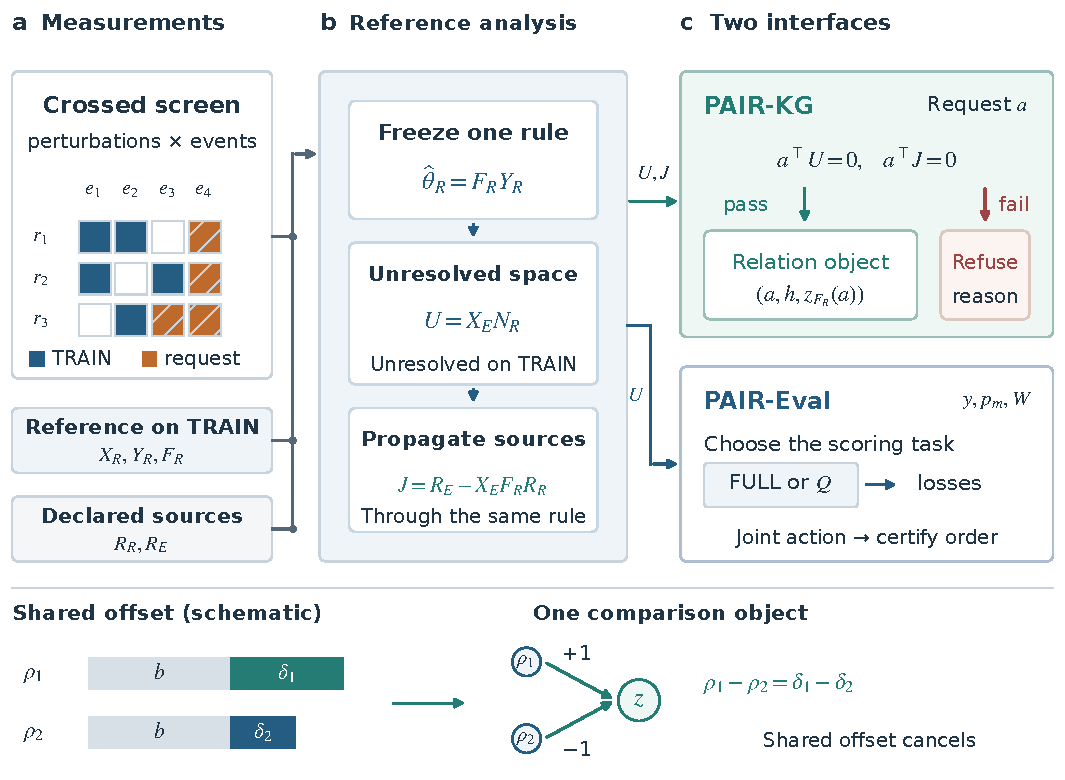
\includegraphics[width=\textwidth]{figures/figure_01.pdf}
\caption{PAIR workflow. Ordered crossed measurements, a TRAIN reference and a registered completion rule define a quantitative contract. PAIR-KG tests and materializes complete signed comparisons with declared-source conditions; the optional PAIR-Eval interface specifies which response component is scored. The lower schematic shows how a comparison can remove a shared offset that remains in its constituent responses. Vector diagram prepared with author-reviewed AI-assisted code.}
\label{fig:overview}
\end{figure}

\section{Related work}\label{sec:related}
\textbf{Estimability in incomplete designs.} Classical linear models and generalized inverses determine the combinations of effects supported by a design~\cite{searle1971linear,rao1971generalized}. In crossed additive tables, graph connectivity supplies a structural characterization; network fixed-effect theory further examines estimation under noise assumptions~\cite{freeman1975incomplete,jochmans2019network}. The \texttt{estimability} package implements numerical estimability tests~\cite{lenth2026estimability}. Matrix completion and recent interpretable-imputation methods instead estimate missing entries under modeling assumptions~\cite{mazumder2010softimpute,vo2026pica}. PAIR uses classical estimability as a component and makes its output a complete, versioned information object.

\textbf{Scientific assertions and provenance.} Knowledge graphs and semantic-unit representations capture associations, statements and context~\cite{hogan2021knowledge,unni2022biolink,vogt2024semanticunits,vogt2026framework}. Provenance representations preserve derivation lineage~\cite{green2007provenance,w3c2013prov,menotti2025provenance,sen2026provsql}. These approaches are compatible with a source-qualified comparison. Our interface makes the statistical cancellation predicate and its numerical completion explicit within the published object, rather than treating provenance as a substitute for a quantitative test.

\textbf{Evaluation under incomplete information.} Decision-informativity results distinguish information sufficient for a decision from information sufficient for full reconstruction~\cite{vanwaarde2020informativity,bennouna2025decision,ye2026decisionsufficient}. Molecular benchmarks emphasize model and scoring comparability~\cite{vinas2026systema,wu2025perturbench,bernett2026dreval}. We therefore separate the qualification of a comparison from the choice of a downstream scoring task. These operations share design geometry but have different empirical success criteria.

\section{Problem formulation}\label{sec:problem}
\subsection{A comparison as an information object}
Let $R$ denote the reference rows drawn from TRAIN and $E$ the ordered rows on which a numerical statement is requested. The observed responses are $Y_R\in\R^{n_R}$ and $Y_E\in\R^{n_E}$; $X_R\in\R^{n_R\times p}$ and $X_E\in\R^{n_E\times p}$ describe the declared additive reference. A query is the \emph{complete} coefficient vector $a\in\R^{n_E}$. The atom selecting one response is a special case; two-term and four-term signed comparisons use several coordinates. The output must retain the vector and the observation ordering that make it meaningful.

We define a versioned measurement contract
\begin{equation}
\mathcal C=\big(R,E,\mathrm{id},X_R,X_E,Y_R,Y_E,F_R,a,R_R,R_E,\tau\big),
\label{eq:contract}
\end{equation}
where $\mathrm{id}$ binds sample and source identities, $F_R$ is a registered linear rule for reference completion, $R_R,R_E$ describe declared additive sources, and $\tau$ specifies numerical tolerances. A downstream evaluation additionally declares an aligned prediction set, scoring support, weights and loss; these are not silently assumed parts of the relation itself.

The \emph{claim-compilation problem} is to map $\mathcal C$ into one of three types of result: (i) a reference- and source-qualified signed comparison with a reproducible value, (ii) a measurement record without assertion authority, or (iii) a refusal naming a failed condition. The scientific quantity is the complete requested comparison. The basic evaluation units are a query on a fixed design, a fold of held-out measurement support, or a fixed-prediction model comparison; repeated queries sharing measurements are not independent experiments.

\subsection{Information-matched comparator}
A correct classical implementation can test the same estimability condition, use the same generalized-inverse completion and propagate the same source maps. Such a pipeline is the appropriate strong comparator; its algebraic qualification decisions are expected to match. PAIR's distinguishable artifact is the explicit, typed \emph{link} among these outputs. Evaluating an implementation advantage would require a native, information-matched comparison of issued records, audit errors, time or memory. Here we test contract consistency, observe the behavior of archived datasets and expose the tasks that still require that experiment.

\section{PAIR: reference- and source-qualified compilation}\label{sec:method}
\subsection{Reference-legal comparisons}
We use the additive decomposition
\begin{equation}
Y_{ij}=\mu+\alpha_i+\beta_j+\Gamma_{ij}+\varepsilon_{ij}
\label{eq:decomp}
\end{equation}
as a working reference model; it does not require all components to be individually estimated. Let $N_R$ span $\ker(X_R)$. Two reference parameter vectors consistent with TRAIN differ along this null space. The requested comparison is estimable with respect to that reference precisely when
\begin{equation}
a^\top X_EN_R=0.
\label{eq:estimable}
\end{equation}
Equivalently, $a^\top X_E$ lies in the row space of $X_R$, so a row-vector $h^\top$ exists satisfying $h^\top X_R=a^\top X_E$. This condition identifies the \emph{comparison}, not necessarily any participating adjusted cell response.

For a fixed reference rule $\widehat\theta_R=F_RY_R$ satisfying $X_RF_RX_R=X_R$, PAIR registers
\begin{equation}
\begin{aligned}
h^\top&=a^\top X_EF_R,\\
z_{F_R}(a)&=a^\top(Y_E-X_EF_RY_R)
           =a^\top Y_E-h^\top Y_R.
\end{aligned}
\label{eq:readout}
\end{equation}
The first equation tests whether the requested linear functional is supported by the reference; the second fixes its finite-data numerical interpretation. Under the model in Eq.~\ref{eq:decomp}, the readout includes $a^\top\Gamma_E-h^\top\Gamma_R$ and the corresponding measurement-error terms. A reported comparison consequently retains its lift $h$, reference version and scale.

\subsection{Propagation of declared shared sources}
Let $u$ denote a vector of declared shared-source contributions entering the reference and requested measurements through matrices $R_R$ and $R_E$. When the registered completion is applied to both measurement and source terms, the residual source map is
\begin{equation}
J=R_E-X_EF_RR_R.
\label{eq:source}
\end{equation}
The source-qualification condition is $a^\top J=0$. Combining it with Eq.~\ref{eq:estimable} gives the complete linear qualification system
\begin{equation}
\boxed{a^\top X_EN_R=0,\qquad a^\top(R_E-X_EF_RR_R)=0.}
\label{eq:jointgate}
\end{equation}
Both tests can be evaluated from design and source metadata before reading the requested outcome values. The numerical readout is calculated only for a qualified query on a fully bound contract.

\begin{proposition}[Composition of the reference and source tests]\label{prop:soundness}
Suppose $Y_R=X_R\theta+\Gamma_R+R_Ru+\varepsilon_R$ and $Y_E=X_E\theta+\Gamma_E+R_Eu+\varepsilon_E$. For a registered $F_R$ satisfying $X_RF_RX_R=X_R$, every query obeying Eq.~\ref{eq:jointgate} has
\begin{equation}
z_{F_R}(a)=a^\top\Gamma_E-h^\top\Gamma_R
+a^\top\varepsilon_E-h^\top\varepsilon_R,
\quad h^\top=a^\top X_EF_R.
\label{eq:soundness}
\end{equation}
\end{proposition}
\noindent\emph{Proof.} Substitute the decompositions into Eq.~\ref{eq:readout}. The additive-reference contribution is $a^\top X_E\theta-h^\top X_R\theta=0$ by estimability and the registered lift. The source term is $a^\top R_Eu-h^\top R_Ru=a^\top Ju=0$. The remaining terms are those in Eq.~\ref{eq:soundness}. $\square$

The result is an algebraic validity statement under the declared linear source map. It motivates a natural separation between \emph{structural eligibility}, \emph{source cancellation}, \emph{reproducible numerical readout} and additional statistical precision analyses.

\subsection{The qualified comparison space and a local witness}
On the requested support write $U=X_EN_R$ and $V=[\,U\ J\,]$. The family of jointly qualified coefficient vectors is
\begin{equation}
\mathcal L_{\mathcal C}=\ker(V^\top),\qquad
Q_{\mathcal C}=I-P_V,
\label{eq:legalspace}
\end{equation}
where $P_V$ is the orthogonal projector onto $\col(V)$. Hence $Q_{\mathcal C}a=a$ is an equivalent test of membership in the legal comparison space. The extra reduction contributed by the declared source map has dimension
\begin{equation}
\delta_{\rm source}=\rank([\,U\ J\,])-\rank(U).
\label{eq:source-increment}
\end{equation}
This representation allows the design factorization to be reused over many requests. For a bound input version $\nu$, the resulting query-local witness contains $(\nu,a,h,z_{F_R}(a))$ and the source-ledger identity. A verifier checks
\begin{equation}
\begin{gathered}
h^\top X_R=a^\top X_E,\qquad
h^\top=a^\top X_EF_R,\\
a^\top R_E=h^\top R_R,\qquad
z_{F_R}(a)=a^\top Y_E-h^\top Y_R.
\end{gathered}
\label{eq:witness}
\end{equation}
The witness records what was checked and the input version against which it was checked. A failure in identity, support, source or numerical agreement returns a typed result (Table~\ref{tab:states}).

\begin{table}[t]
\centering\small
\caption{Compiler outputs: each status describes the requested assertion, not the biological absence of an effect.}
\label{tab:states}
\begin{tabularx}{\textwidth}{@{}L{0.32\textwidth}X@{}}
\toprule
Output & Information conveyed \\\midrule
\texttt{COMPARATIVE\_ASSERTABLE} & Signed query, reference completion, declared source map and value are bound and pass checks.\\
\texttt{NOT\_IDENTIFIABLE} & The TRAIN reference leaves a component of the signed query unresolved.\\
\texttt{SOURCE\_UNSAFE} & A declared source contribution survives the registered completion.\\
\texttt{NUMERICALLY\_UNRESOLVED} & Independent numerical checks disagree at the registered tolerance.\\
\texttt{MEASUREMENT\_ONLY} & The measurement can be retained, but assertion inputs or certification are incomplete.\\
\bottomrule
\end{tabularx}
\end{table}

\subsection{Two instructive cases}
\textbf{Why the completion identity matters.} Take $X_R=(1,1)^\top$, $Y_R=(0,2)^\top$, $X_E=(1)$, $Y_E=3$, $a=1$, and declared sources $R_R=(1,0)^\top$, $R_E=(1)$. The query passes the reference test. Two generalized-inverse completions $F_1=(1,0)$ and $F_2=(0,1)$ both satisfy the reference equation, but Eq.~\ref{eq:readout} gives $z_{F_1}=3$ and $z_{F_2}=1$; Eq.~\ref{eq:source} gives $J_1=0$ and $J_2=1$. A source decision made with one completion cannot be attached to the value obtained from the other. This constructed example isolates the cross-interface requirement that PAIR records explicitly.

\textbf{A completion-independent special case.} In a strict $2\times2$ additive contrast with coefficients $(+1,-1,-1,+1)$, the full query satisfies $a^\top X_E=0$. Thus $h=0$, $z_{F_R}(a)=a^\top Y_E$ and $a^\top J=a^\top R_E$ for every registered linear completion. The reference part of this comparison is already eliminated by its coefficients. This special case is central to interpreting the Replogle results: when the declared shared control also cancels, a source check adds no further rejection. The general compiler nevertheless distinguishes it from queries whose value depends on an explicit reference lift (Supplementary Sections S1 and S16).

\begin{proposition}[When the completion can change a claim]\label{prop:operator-independence}
Let $w^\top=a^\top X_E$ be reference-legal and let $\mathfrak F(X_R)=\{F:X_RFX_R=X_R\}$ be the family of admissible generalized-inverse completions. On fixed measured inputs, the pair
\[
\big(z_F(a),\ a^\top R_E-w^\top FR_R\big)
\]
is independent of the choice $F\in\mathfrak F(X_R)$ if and only if $w=0$ or every column of $[\,Y_R\ R_R\,]$ belongs to $\col(X_R)$.
\end{proposition}
\noindent\emph{Reason.} If $w=0$ both quantities are independent of $F$. If $[Y_R\ R_R]=X_RB$, generalized-inverse consistency makes $w^\top FX_RB$ unique. Conversely, when $w\ne0$ and a column lies outside $\col(X_R)$, perturbing a generalized inverse by $u q^\top$ with $q\in\ker(X_R^\top)$ changes the corresponding completed term while leaving $X_RFX_R=X_R$. Section S16 gives the complete proof and exact-rational checks. The result identifies when completion binding is a substantive numerical requirement and when a strict additive comparison already fixes the answer.

\subsection{Compilation and downstream evaluation}\label{sec:evaltask}
Implementation proceeds by binding the ordered input version, factorizing the TRAIN design, checking Eqs.~\ref{eq:jointgate} and~\ref{eq:witness}, and emitting the qualified record or a typed outcome. The reference null space and source map are reused for requests sharing one design. Numerical rank is checked with independent SVD and pivoted-QR routes at fixed tolerances. The contract follows the deterministic order in Table~\ref{tab:compiler}; factorization and numerical defaults are detailed in S1--S2.

\begin{table}[t]
\centering\small
\caption{Compiler steps for a fixed TRAIN and source-contract version.}
\label{tab:compiler}
\begin{tabularx}{\textwidth}{@{}L{0.16\textwidth}X@{}}
\toprule
Stage & Operation and observable output \\\midrule
Bind & Validate ordered sample/source identities, response scale, $F_R$ and numerical tolerances.\\
Factorize & Obtain $N_R$, $U=X_EN_R$ and $J=R_E-X_EF_RR_R$ once per fixed support.\\
Qualify & Test $a^\top U=0$ and $a^\top J=0$; otherwise return a typed status.\\
Read out & Compute $h^\top=a^\top X_EF_R$ and $z=a^\top Y_E-h^\top Y_R$.\\
Verify & Check Eq.~\ref{eq:witness} through an independent numerical path.\\
Publish & Emit the complete comparison, source and reference bindings, status and witness.\\
\bottomrule
\end{tabularx}
\end{table}

The same design geometry can define an optional evaluation target. Let $U=X_EN_R$ on a matched evaluation support and $Q=I-P_U$. For predictions $p_m$ aligned to observed responses $y$, the \emph{identified-component} squared loss uses $\|Q(y-p_m)\|_2^2$, whereas full-response scoring uses $\|y-p_m\|_2^2$. With an orthogonal projector and common unweighted support,
\begin{equation}
\|y-p_m\|_2^2=\|Q(y-p_m)\|_2^2+\|(I-Q)(y-p_m)\|_2^2.
\label{eq:scoredecomp}
\end{equation}
Both losses are legitimate but answer different evaluation questions. A source-restricted task may instead use $Q_{\mathcal C}$ in Eq.~\ref{eq:legalspace}, provided the corresponding source identities are bound. The score comparison is thus explicitly downstream of, and conceptually distinct from, compiling a quantitative claim. Joint actions and decision-information certificates are derived in S5 and S14.

\section{Evaluation protocol}\label{sec:study}
\subsection{Datasets, units and preregistered decisions}
We use the frozen K562 APA regulator--event screen~\cite{kowalski2024cpa}, ENCODE RBP--splicing supports~\cite{vannostrand2020rbp}, independent HEK293T PAS-seq event folds~\cite{jagannatha2026rbp}, Replogle K562 Perturb-seq native metadata~\cite{replogle2022perturbseq}, and fixed drug-response predictions for CTRPv2 and GDSC~\cite{rees2016ctrp,iorio2016gdsc,bernett2026dreval}. The experiments ask whether complete comparisons survive missing atomic support, whether declared-source mappings preserve their eligibility, and whether a declared change of scoring target alters decisions on fixed predictions. Source and reference gates are specified using TRAIN and metadata before requested response values are read.

\begin{table}[t]
\centering\small
\caption{Experimental units and evaluation targets. Query counts, split exposures and cell identities are reported separately.}
\label{tab:resources}
\begin{tabularx}{\textwidth}{@{}L{0.22\textwidth}L{0.31\textwidth}X@{}}
\toprule
Resource & Unit or support & Evaluation target \\\midrule
K562 APA & 150 inner-split exposures; separate fold-0 panel with 3,125 requests & Composite legal dimensions and archived query readouts\\
ENCODE RBP--splicing & 20 fixed masks & Legal comparison dimensions under missing support\\
HEK293T PAS-seq & Five strict new-event folds & Replicate-common legal contrast structure\\
Replogle Perturb-seq & 310,385 cell identities; fixed 256-gene panel & Source-bound four-term query \emph{designs}\\
CTRPv2 LDO & Seven fixed-prediction models, 10 folds & FULL versus identified-component rankings\\
GDSC2/GDSC1 LDO & Six primary models per resource, 10 folds & Prespecified persistent ranking reversal\\
Symmetric HPO & One new training realization, 560 jobs & Reproducibility of archived directed reversals\\
\bottomrule
\end{tabularx}
\end{table}

For the drug-response study, a directed pair--metric reversal is persistent when it has the same direction in at least seven of ten folds. The primary GDSC2 endpoint requires both median reversal fraction at least 0.10 and one persistent pair--metric result. These thresholds remain unchanged in the analyses below. The many four-cell requests in crossed screens share regulators, events or controls, so we report them as overlapping query instances.

\subsection{Fair comparators and reported endpoints}
We distinguish four comparators. (1) A query-type shortcut ignores TRAIN support and is a stress-test control. (2) Classical graph connectivity and row-space estimability receive the same support and must agree on exact legal labels. (3) Registered generalized-inverse/OLS completion plus the same source ledger implements an information-matched algebraic comparator. (4) A native, end-to-end classical record producer would additionally consume authenticated input identities, generate identical output schemas and permit time, memory and error-rate comparisons; those original source payloads are not yet complete for this final test. Consequently, results below report \emph{label agreement}, \emph{readout reproducibility}, \emph{source-filter changes} and \emph{evaluation-task sensitivity} rather than an invented percentage improvement in predictive accuracy.

\section{Results}\label{sec:results}
\subsection{Compound comparisons survive missing atomic support}
On 150 K562 inner-split exposures, 9,945 requested adjusted-effect instances lack atomic support, while 2,635 dimensions remain estimable only as composites after a rank increment of 7,310. These composite-only dimensions represent 26.50\% of the unsupported coordinate exposures. The 20 ENCODE masks analogously contain 973,298 unsupported coordinate instances, a rank increment of 916,903 and 56,395 composite-only dimensions (5.79\%). Every examined K562 and ENCODE support contains a nonempty legal composite subspace (Fig.~\ref{fig:internal}a). These are rank properties of frozen designs, not counts of independent biological discoveries.

The saved K562 and HEK293T replicate channels provide a complementary numerical check. For a legal source-safe basis $B$, set $G=(BB^\top)^{-1}$ and let $z_1,z_2$ be completed responses on two channels. The basis-invariant statistic $\widehat S=z_1^\top Gz_2/\rank(B)$ is positive in five K562 folds (0.082--0.128) and five HEK293T folds (0.026--0.054). Source-safe dimensions range from 2,017 to 2,505 and from 4,927 to 5,593, respectively (Fig.~\ref{fig:internal}b). This establishes measurable aggregate structure in the identified space using the frozen analysis units.

\begin{figure}[t]
\centering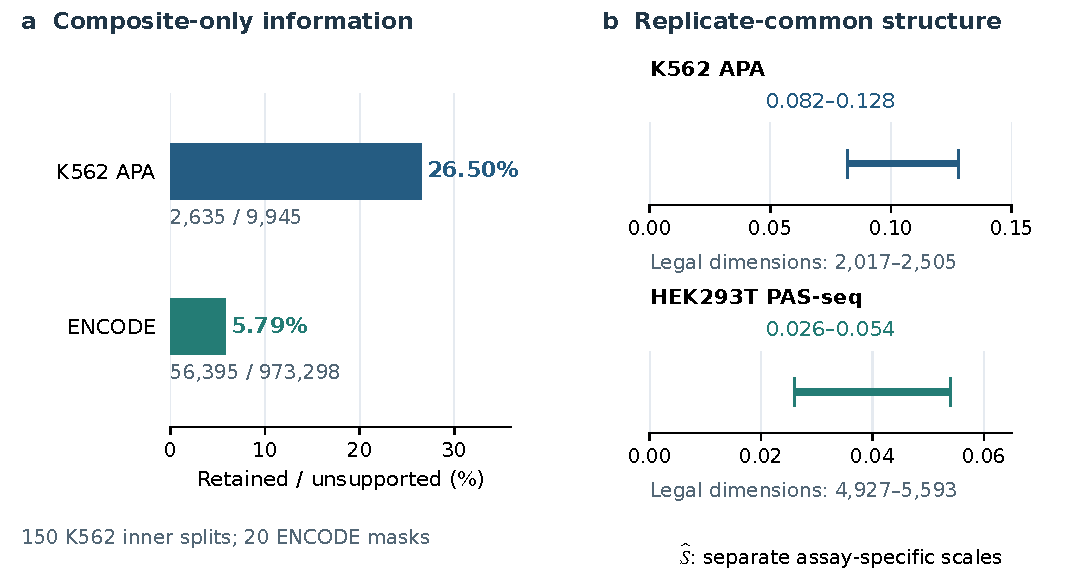
\includegraphics[width=\textwidth]{figures/figure_02.pdf}
\caption{Comparison information in frozen molecular-screen designs. (a) Unsupported adjusted-response coordinates and surviving composite-only dimensions for K562 and ENCODE. (b) Replicate-common summaries and source-safe dimension ranges over five strict new-event folds in K562 and HEK293T. Fold ranges are descriptive, and each assay retains its own response scale. Plot prepared with author-reviewed AI-assisted code.}
\label{fig:internal}
\end{figure}

The separate historical K562 fold-0 producer stored 349 comparative statuses and 2,776 nonidentifiable statuses among 3,125 requests. A processed-data reconstruction using \texttt{consensus\_effect}, a fixed OLS rule and TRAIN membership inferred retrospectively from Q1 identities reproduces all 3,125 stored labels and all 349 numerical readouts, with maximum absolute discrepancy about $2.3\times10^{-14}$. This establishes the numerical consistency of the recovered rule on the inferred support. The original per-query source matrices, producer call lineage and independently sealed TRAIN membership are not included in that reconstruction. We therefore report the 349 as historical compiled records; original source qualification remains a separate provenance test (S6, S10, S15).

\subsection{Source qualification in the Replogle design}
The Replogle source contract is defined on raw cell identities. It records library-size normalization independent of controls, pseudobulk aggregation, and subtraction of a shared control. The metadata universe contains 310,385 valid cells, 8,563 measured genes and 48 GEM groups. The roster contains 97 non-targeting guide \emph{identities}. A fixed 256-gene panel supplies 100,000 overlapping four-term query structures whose support and source geometry are evaluated before expression readout (Fig.~\ref{fig:replogle}).

\begin{figure}[t]
\centering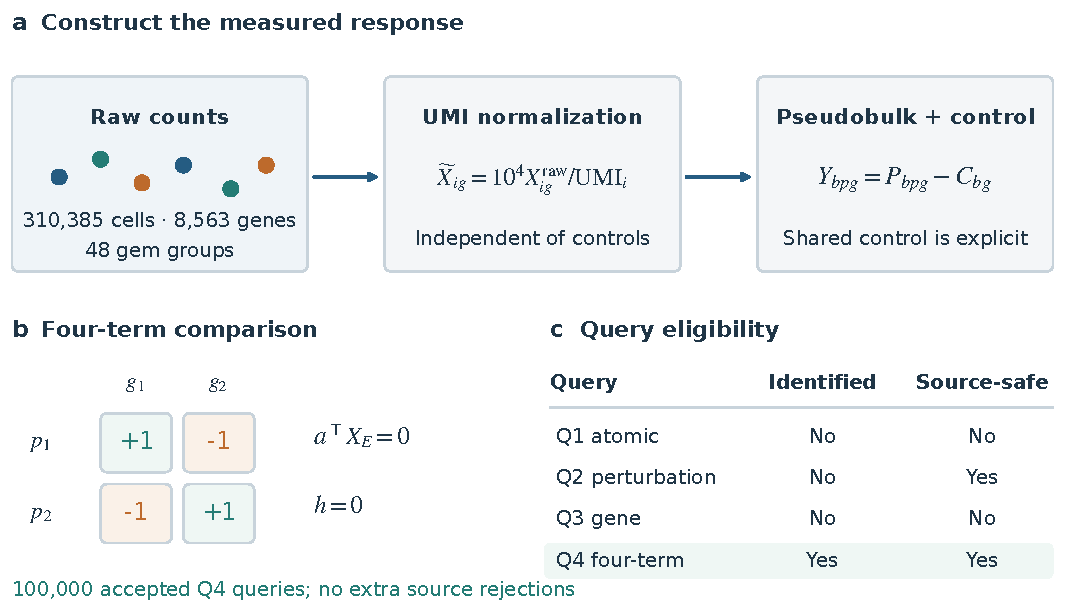
\includegraphics[width=\textwidth]{figures/figure_03.pdf}
\caption{Replogle source contract and four-cell geometry. (a) Declared raw-count, library normalization and shared-control flow. (b) Additive row and column terms cancel in a complete four-term comparison. (c) All 100,000 overlapping query designs satisfy the registered reference and source predicates; these results are eligibility checks on metadata and declared transformations, rather than 100,000 new expression measurements. Plot prepared with author-reviewed AI-assisted code.}
\label{fig:replogle}
\end{figure}

All 100,000 query \emph{designs} pass the reference and declared-source gates. In this equal-weight construction, the complete four-term coefficient vector cancels the shared control automatically, yielding $\delta_{\rm source}=0$. Thus the source test has no incremental exclusions and the completion-independent identity from Section~\ref{sec:method} applies. The original approximately 10-GB expression matrix was not reprocessed to calculate 100,000 new effect estimates. This result establishes a large-scale eligibility pattern for a stated source transformation and identifies the precise case in which source qualification is redundant.

\subsection{Classical controls and implementation comparisons}
A saved K562 fold-0 table has 2,744 Q1 requests (0 accepted), 222 Q2 (222 accepted), 32 Q3 (0 accepted) and 127 Q4 (127 accepted). On that specific table, query type alone reproduces the archived labels. Across 50 other outer-mask supports, all TRAIN bipartite graphs are connected; in 10,182,954 highly overlapping requests, a query-type shortcut matches the actual design labels in 24.10\% of cases. Exact graph/row-space analysis gives the correct structural classification, and deterministic graph deletions expose within-type failures of the shortcut. These comparisons place the compiler's legality rule on the classical design-theory baseline, not above it (S10--S11).

For predictive controls, a low-dimensional B2 baseline on 50 frozen K562 masks reduces MSE from 0.1905898683 (zero D3) to 0.1129436318 (40.740\% reduction; reported 95\% interval 33.106--46.961\%). The more specific rank-four comparison-supervision diagnostic gives average calibrated TEST losses of 0.8354 for ordinary supervision and 0.8364 for four-term supervision, with the zero-interaction comparator at 1.0000. Both analyses use their original frozen training/evaluation contracts (S3, S8).

\begin{table}[t]
\centering\small
\caption{Information-matched comparisons and observed incremental differences. Dashes denote endpoints for which no native matched estimate is available.}
\label{tab:fair}
\begin{tabularx}{\textwidth}{@{}L{0.26\textwidth}L{0.32\textwidth}X@{}}
\toprule
Question / comparator & Observed comparison & Interpretation \\\midrule
Reference legality: graph or row-space & Same structural labels on matched support & Established exact comparator agrees\\
Type-only shortcut & 24.10\% agreement on 10,182,954 dependent outer-mask queries & Support identities matter\\
Replogle source increment & $\delta_{\rm source}=0$ for registered Q4 structures & No incremental source refusals\\
Contrast-supervised versus ordinary predictor & Calibrated TEST loss 0.8364 versus 0.8354 & No observed gain from contrast supervision\\
Exact decision LP (supplement) & Pairwise scheme 43 calls; classical comparator 42 & Equivalent task, no efficiency gain\\
Native classical assertion producer & Original matched source payload incomplete & End-to-end performance undetermined\\
\bottomrule
\end{tabularx}
\end{table}

\subsection{Changing the scoring target changes some model decisions}
For drug-response evaluation, $Q$ removes TRAIN-unresolved directions from matched residuals. Full-response and identified-component losses are different targets by Eq.~\ref{eq:scoredecomp}. The official frozen CTRPv2 leave-drug-out predictions exhibit median pairwise reversal fractions of 0.50 for normalized $R^2$ and 0.357 for normalized Pearson (Fig.~\ref{fig:drug}). Five directed pair--metric outcomes involving four non-naive model pairs reverse in at least seven of ten folds. By ten-fold arithmetic mean, the normalized-$R^2$ leader changes from MultiOmicsNeuralNetwork to DIPK when the scored component changes. A common-support review retains 102 of 210 normalized-$R^2$ model-pair--fold reversals: 55 native-common-support and 47 recorded transport-category cases; the independent scorer reproduces the recorded 210 signs (S4, S6).

\begin{figure}[t]
\centering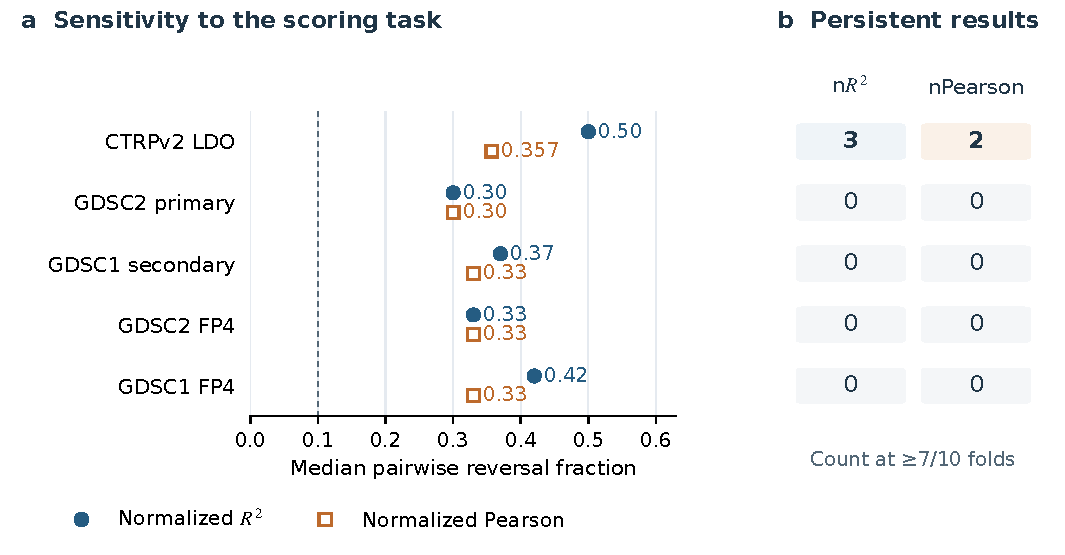
\includegraphics[width=\textwidth]{figures/figure_04.pdf}
\caption{Task-dependent model order. (a) Median pairwise order-reversal fractions between FULL and identified-component scoring. (b) Number of model pair--metric outcomes with the same directed reversal in at least 7/10 folds. The primary GDSC2 and the GDSC1/FP4 controls contain zero persistent outcomes under this criterion. Plot prepared with author-reviewed AI-assisted code.}
\label{fig:drug}
\end{figure}

External confirmation is more restrictive. In GDSC2 the median reversal fractions are 0.30 for normalized $R^2$ and 0.30 for Pearson, but no directed pair--metric result persists in at least seven folds. GDSC1 shows 0.37/0.33 and again zero persistence; enlarged FP4 supports also produce zero persistent outcomes. The prespecified GDSC2 condition therefore fails. In one separate symmetric-HPO training realization covering 560 training/final-prediction jobs, the five historical reversal counts (7/7/8/7/7) become 5/6/7/6/5; one of the five meets the original threshold (Supplementary Section S4). These tests identify a task-sensitive score but do not yield a stable cross-resource model ordering.

\section{Discussion}\label{sec:discussion}
The main practical object in PAIR is a \emph{qualified comparison}, not a filled table. The distinction matters when the data retain a comparison but not the adjusted responses from which an ordinary database row might be assembled. The signed coefficients, reference lift and source identity specify a reusable numerical statement. The local witness permits a recipient to check its declared algebraic obligations, while typed outcomes preserve an unsupported measurement without converting it into a false negative claim. Completion-dependent queries require particularly careful binding: the constructed example changes both the value and source decision when the completion changes. Strict additive four-cell comparisons, by contrast, expose a useful simplification---their numerical value can be independent of the reference completion.

The empirical evaluation illustrates three complementary properties. The frozen K562 and ENCODE supports retain composite information; the Replogle templates demonstrate source-bound design qualification but no added exclusions for the declared shared control; and fixed drug-response predictions show that a different scored response component can change ranking. The corresponding exact classical tests are part of the intended specification. For any identical reference, completion and source map, a properly composed classical implementation reaches the same algebraic decision. The empirical contribution here is the joint contract and its observed use across datasets, not a claimed new rank estimator or universal scoring improvement.

Several limitations define the next evaluation step. The original K562 query producer's aligned source matrices and TRAIN provenance are required for independent source-native certification of the 349 historical records. The Replogle qualification results concern query designs, pending expression-level readouts and biological validation. A matched end-to-end classical assertion producer has not yet been measured for time, memory or audit-error reduction, and the GDSC2 persistence test is negative. These issues are stated once because they concern distinct validation targets: historical provenance, measured biological utility, implementation performance and out-of-resource scoring stability. Supplementary Sections S10--S16 retain the stress tests, alternative source granularities, precision checks, and dependent-query reliability analyses.

\section{Conclusion}
PAIR describes an information interface for compiling complete, reference- and source-qualified quantitative comparisons from incomplete molecular screens. It couples an estimability predicate to a fixed numerical lift, a declared source map and a versioned witness. The frozen experiments demonstrate retained composite comparison spaces, conditional reconstruction of archived query values, source eligibility under a strict four-cell design, and task-dependent model evaluation. The resulting contribution is an explicit contract for what a quantitative statement means when it leaves the original analysis pipeline. Future native-source and matched-workflow measurements will determine whether that specification also yields a measurable end-to-end operational advantage.

\section*{Data and code availability}
Supplementary Code S1 contains the editable manuscript source, vector figures, exact algebraic checks and an input-bound quantitative-comparison verifier. The underlying K562, ENCODE, Replogle, CTRPv2 and GDSC resources are identified through the cited primary studies and should be obtained from their original providers under the applicable access terms. The software archive includes a coverage manifest that distinguishes the supplied checks from archived producer inputs and frozen evaluation files that are not redistributed with this snapshot.

\section*{CRediT authorship contribution statement}
\AuthorContributions
\section*{Funding}
\FundingStatement
\section*{Declaration of competing interest}
The authors declare no relevant financial or non-financial competing interests.
\section*{Declaration of generative AI and AI-assisted technologies in the manuscript preparation process}
During manuscript preparation, the authors used OpenAI ChatGPT and coding assistants for language editing, text organization, LaTeX preparation, verification-script assistance and vector-diagram code. The authors reviewed and edited the resulting material, verified numerical statements against their available research records, and take responsibility for the content. The writing revision did not alter the frozen measurements, predictions or prespecified evaluation decisions.

\begingroup\small\setstretch{1.0}
\bibliographystyle{unsrtnat}
\bibliography{references}
\endgroup
\end{document}
